\documentclass[11pt,a4paper,twocolumn]{article}
\usepackage[utf8]{inputenc}
\usepackage[T1]{fontenc}
\usepackage{amsmath,amssymb,amsthm}
\usepackage{tikz}
\usetikzlibrary{arrows,arrows.meta,positioning,calc,shapes.geometric,decorations.markings}
\usepackage[margin=1cm,footskip=0.5cm]{geometry}
\usepackage{enumitem}
\usepackage{hyperref}
\usepackage{tocloft}
\usepackage{graphicx}
\usepackage{algorithm}
\usepackage{algpseudocode}
\usepackage{float}
\usepackage{placeins}
\usepackage{tabularx}

% Column separator and spacing
\setlength{\columnseprule}{0.4pt}
\setlength{\columnsep}{1cm}

% Better paragraph and page breaks
\widowpenalty=10000
\clubpenalty=10000
\raggedbottom

% Float control
\setcounter{topnumber}{4}
\setcounter{bottomnumber}{4}
\setcounter{totalnumber}{10}
\renewcommand{\topfraction}{0.9}
\renewcommand{\bottomfraction}{0.9}
\renewcommand{\textfraction}{0.1}
\renewcommand{\floatpagefraction}{0.7}

% Remove section numbers from TOC
\setcounter{tocdepth}{3}
\setcounter{secnumdepth}{3}

% Title settings
\title{\textbf{FTP\_Algorithms}\\
       \large Cheat Sheet}
\author{Diego Gil}
\date{Herbstsemester 2024/25}

\tikzset{
    >={Stealth[]},
    every picture/.style={line width=0.5pt},
    vertex/.style={circle,draw,minimum size=20pt,inner sep=0pt}
}

\begin{document}
\onecolumn
\maketitle

\twocolumn
\tableofcontents
\newpage

\clearpage

% Content from weeks 1-7
\clearpage
\section{\texorpdfstring{\underline{Search and Analysis}}{Search and Analysis}}

\clearpage
\section{\texorpdfstring{\underline{Data Structures}}{Data Structures}}
\subsection{Trees}
\subsubsection{Basic Tree Terminology}
\textbf{Height:} The height of a tree is the length of the longest path from the root to a leaf. It is the number of edges on this path.

\textbf{Level:} The level of a node is the number of edges on the path from the root to the node. The root node is at level 0.

\textbf{Minimum Width:} The minimum width of a tree is the smallest number of nodes at any level of the tree.

\textbf{Maximum Width:} The maximum width of a tree is the largest number of nodes at any level of the tree.

\textbf{Depth:} The depth of a node is the number of edges from the node to the tree's root node.

\textbf{Leaf:} A leaf is a node with no children.

\textbf{Internal Node:} An internal node is a node with at least one child.

\textbf{Binary Tree:} A tree data structure in which each node has at most two children, referred to as the left child and the right child.

\subsubsection{KD-Trees}
\textbf{Problem Type:} Construction of a KD-Tree from 2D points

\textbf{What to Look For:}
\begin{itemize}[noitemsep,leftmargin=*]
    \item Set of 2D points given as coordinates
    \item Request to build a KD-Tree
    \item Questions about tree properties (height, leaves)
\end{itemize}

\textbf{Given Points:} 
$P = \{(1,3), (12,1), (4,5), (5,4),$ \\
\hspace*{1cm} $(10,11), (8,2), (2,7)\}$

\textbf{Solution Strategy:}
\begin{enumerate}[leftmargin=*,noitemsep]
    \item Sort points by x-coordinate (root level)
    \item Find median point
    \item Split into left/right subtrees
    \item Repeat with y-coordinates for next level
    \item Continue alternating x/y until all points placed
\end{enumerate}

\textbf{Detailed Solution:}
\begin{enumerate}[leftmargin=*,label=\arabic*.]
    \item \textbf{Root Level (x-split)}
    \begin{itemize}[noitemsep]
        \item Sorted x: \\
        $(1,3), (2,7), (4,5),$ \\
        $\mathbf{(5,4)},$ \\
        $(8,2), (10,11), (12,1)$
        \item Median $(5,4)$ becomes root $\ell_1$
    \end{itemize}

    \begin{figure}[H]
    \centering
    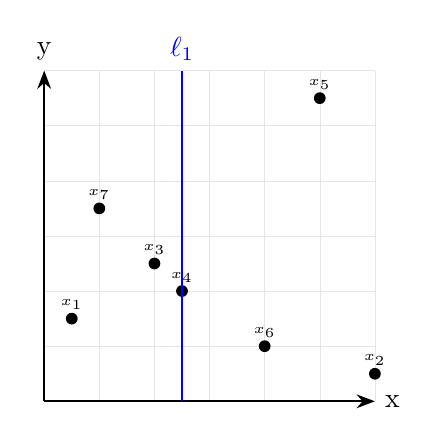
\begin{tikzpicture}[scale=0.35]
        % Grid
        \draw[very thin,gray!20] (0,0) grid[step=2] (12,12);
        \draw[->,thick] (0,0) -- (12,0) node[right] {x};
        \draw[->,thick] (0,0) -- (0,12) node[above] {y};
        
        % Points with labels
        \foreach \x/\y/\label in {
            1/3/1, 12/1/2, 4/5/3, 5/4/4, 10/11/5, 8/2/6, 2/7/7
        } {
            \node[circle,fill,inner sep=1.5pt] at (\x,\y) {};
            \node[font=\tiny] at (\x,\y+0.5) {$x_{\label}$};
        }
        
        % Splitting line
        \draw[blue,thick] (5,0) -- (5,12) node[above] {$\ell_1$};
    \end{tikzpicture}
    \caption*{Coordinate Split at Root Level}
    \end{figure}

    \item \textbf{Tree Structure}
    \begin{figure}[H]
    \centering
    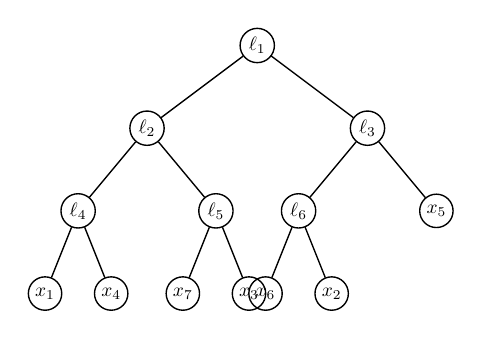
\begin{tikzpicture}[
        level distance=1.5cm,
        level 1/.style={sibling distance=4cm},
        level 2/.style={sibling distance=2.5cm},
        level 3/.style={sibling distance=1.2cm},
        scale=0.7,
        every node/.style={transform shape}
    ]
    \node [circle,draw,inner sep=2pt] {$\ell_1$}
        child {node [circle,draw,inner sep=2pt] {$\ell_2$}
            child {node [circle,draw,inner sep=2pt] {$\ell_4$}
                child {node [circle,draw,inner sep=2pt] {$x_1$}}
                child {node [circle,draw,inner sep=2pt] {$x_4$}}
            }
            child {node [circle,draw,inner sep=2pt] {$\ell_5$}
                child {node [circle,draw,inner sep=2pt] {$x_7$}}
                child {node [circle,draw,inner sep=2pt] {$x_3$}}
            }
        }
        child {node [circle,draw,inner sep=2pt] {$\ell_3$}
            child {node [circle,draw,inner sep=2pt] {$\ell_6$}
                child {node [circle,draw,inner sep=2pt] {$x_6$}}
                child {node [circle,draw,inner sep=2pt] {$x_2$}}
            }
            child {node [circle,draw,inner sep=2pt] {$x_5$}}
        };
    \end{tikzpicture}
    \caption*{KD-Tree Structure}
    \end{figure}
    \FloatBarrier

    \item \textbf{Final Properties}
    \begin{itemize}[noitemsep,leftmargin=*]
        \item Height: 3 (counting from 0)
        \item Leaves: 7 (all original points)
        \item Second leaf from left: $(4,5)$
    \end{itemize}
\end{enumerate}

\textbf{Exam Tips:}
\begin{enumerate}[noitemsep,leftmargin=*]
    \item Always start by sorting points on current dimension
    \item Mark median point clearly in your sorting
    \item Draw coordinate system with splitting lines
    \item Keep track of which dimension you're splitting on:
        \begin{itemize}[noitemsep,topsep=0pt]
            \item Level 0: x-coordinate
            \item Level 1: y-coordinate
            \item Level 2: x-coordinate
            \item And so on...
        \end{itemize}
    \item Verify tree properties at the end
\end{enumerate}

\textbf{Common Mistakes to Avoid:}
\begin{itemize}[noitemsep,leftmargin=*]
    \item Don't forget to alternate dimensions
    \item Don't skip sorting at each level
    \item Don't mix up left (<) and right (>) subtrees
    \item Don't forget to verify final tree properties
\end{itemize}

\FloatBarrier

\subsubsection{KD-Tree Complexity Analysis}
\textbf{Problem Type:} Complexity proof for KD-Tree construction

\textbf{What to Look For:}
\begin{itemize}[noitemsep,leftmargin=*]
    \item Proof of time complexity $O(n\log n)$
    \item Proof of space complexity $O(n)$
    \item Recursive analysis
\end{itemize}

\textbf{Solution Strategy:}
\begin{enumerate}[leftmargin=*,noitemsep]
    \item Prove space complexity first (easier)
    \item Analyze recursive structure
    \item Set up recurrence relation
    \item Apply Master Theorem
\end{enumerate}

\textbf{Space Complexity Proof:}
\begin{enumerate}[leftmargin=*,noitemsep]
    \item For $n = 2^k$ points:
        \begin{itemize}[noitemsep,topsep=0pt]
            \item Internal nodes (parents): $2^k - 1$
            \item Total nodes: $2^k + 2^{k-1} = n + n/2 = 3n/2 < 3n$
        \end{itemize}
    \item For general $n$ (not power of 2):
        \begin{itemize}[noitemsep,topsep=0pt]
            \item Find $t$ where $2^{t-1} < n < 2^t$
            \item Internal nodes $n_p$: $2^{t-2} < n_p < 2^{t-1}$
            \item Total nodes: $3 \cdot 2^{t-2} < n + n_p < 3 \cdot 2^{t-1}$
            \item Therefore: $n + n_p < 3n$
        \end{itemize}
    \item Each node uses $O(1)$ storage
    \item Total storage: $O(1) \cdot O(n) = O(n)$
\end{enumerate}

\textbf{Time Complexity Proof:}
\begin{enumerate}[leftmargin=*,noitemsep]
    \item At each recursion:
        \begin{itemize}[noitemsep,topsep=0pt]
            \item Split $n$ points into two subsets of $n/2$
            \item Finding median costs $O(n)$
        \end{itemize}
    \item Recurrence relation:
        \[ T(n) = \begin{cases}
            O(1) & \text{if } n = 1 \\
            2T(n/2) + O(n) & \text{if } n > 1
        \end{cases} \]
    \item Apply Master Theorem:
        \begin{itemize}[noitemsep,topsep=0pt]
            \item Similar to Merge-Sort analysis
            \item Results in $T(n) = O(n\log n)$
        \end{itemize}
\end{enumerate}

\textbf{Key Points for Exam:}
\begin{itemize}[noitemsep,leftmargin=*]
    \item Space complexity proof:
        \begin{itemize}[noitemsep,topsep=0pt]
            \item Count nodes for power of 2
            \item Extend to general case
            \item Multiply by constant storage
        \end{itemize}
    \item Time complexity proof:
        \begin{itemize}[noitemsep,topsep=0pt]
            \item Identify recursive pattern
            \item Write recurrence relation
            \item Apply Master Theorem
        \end{itemize}
    \item Remember median finding is $O(n)$
\end{itemize}

\textbf{Common Mistakes to Avoid:}
\begin{itemize}[noitemsep,leftmargin=*]
    \item Don't forget to account for non-power-of-2 cases
    \item Don't ignore constant factors in space analysis
    \item Remember to justify linear median finding
    \item Don't skip the Master Theorem application
\end{itemize}

\FloatBarrier

\subsubsection{Binary Search Trees (BST)}
\textbf{Definition:} A binary tree where for each node $x$:
\begin{itemize}[noitemsep,leftmargin=*]
    \item All keys in left subtree are < $x.key$
    \item All keys in right subtree are > $x.key$
    \item No duplicate keys allowed
\end{itemize}

\textbf{Basic Operations:}
\begin{enumerate}[noitemsep,leftmargin=*]
    \item \textbf{TREE-SEARCH$(x,k)$}: Find node with key $k$
        \begin{itemize}[noitemsep,topsep=0pt]
            \item Start at root, compare with $k$
            \item If equal: found
            \item If $k$ smaller: go left
            \item If $k$ larger: go right
            \item Time: $O(h)$ where $h$ is height
        \end{itemize}
    
    \item \textbf{TREE-MINIMUM$(x)$}: Find smallest key
        \begin{itemize}[noitemsep,topsep=0pt]
            \item Follow left pointers until NIL
            \item Time: $O(h)$
        \end{itemize}
    
    \item \textbf{TREE-MAXIMUM$(x)$}: Find largest key
        \begin{itemize}[noitemsep,topsep=0pt]
            \item Follow right pointers until NIL
            \item Time: $O(h)$
        \end{itemize}
    
    \item \textbf{TREE-SUCCESSOR$(x)$}: Find next larger key
        \begin{itemize}[noitemsep,topsep=0pt]
            \item If right subtree exists: TREE-MINIMUM(right)
            \item Else: Go up until first right turn
            \item Time: $O(h)$
        \end{itemize}
    
    \item \textbf{TREE-PREDECESSOR$(x)$}: Find next smaller key
        \begin{itemize}[noitemsep,topsep=0pt]
            \item If left subtree exists: TREE-MAXIMUM(left)
            \item Else: Go up until first left turn
            \item Time: $O(h)$
        \end{itemize}
\end{enumerate}

\textbf{Modifying Operations:}
\begin{enumerate}[noitemsep,leftmargin=*]
    \item \textbf{TREE-INSERT$(T,z)$}: Insert new node $z$
        \begin{itemize}[noitemsep,topsep=0pt]
            \item Follow BST property down to leaf
            \item Insert as left/right child
            \item Time: $O(h)$
        \end{itemize}
    
    \item \textbf{TREE-DELETE$(T,z)$}: Delete node $z$
        \begin{itemize}[noitemsep,topsep=0pt]
            \item Case 1: No children - remove directly
            \item Case 2: One child - replace with child
            \item Case 3: Two children:
                \begin{itemize}[noitemsep,topsep=0pt]
                    \item Find successor $y$ (min in right subtree)
                    \item Replace $z$ with $y$
                    \item Delete $y$ from original position
                \end{itemize}
            \item Time: $O(h)$
        \end{itemize}
\end{enumerate}

\textbf{Helper Operation:}
\begin{itemize}[noitemsep,leftmargin=*]
    \item \textbf{TRANSPLANT$(T,u,v)$}: Replace subtree
        \begin{itemize}[noitemsep,topsep=0pt]
            \item Replaces subtree rooted at $u$ with subtree rooted at $v$
            \item Updates parent pointers
            \item Used in DELETE operation
        \end{itemize}
\end{itemize}

\textbf{Properties:}
\begin{itemize}[noitemsep,leftmargin=*]
    \item Inorder traversal gives sorted sequence
    \item Height $h$ determines operation time:
        \begin{itemize}[noitemsep,topsep=0pt]
            \item Best case (balanced): $h = \lg n$
            \item Worst case (linear): $h = n$
        \end{itemize}
    \item No explicit balancing - shape depends on insertion order
\end{itemize}

\textbf{Tree Traversal:}
\begin{itemize}[noitemsep,leftmargin=*]
    \item \textbf{Inorder}: Left subtree → Root → Right subtree
        \begin{itemize}[noitemsep,topsep=0pt]
            \item Visits nodes in sorted order
            \item Used for ordered printing
        \end{itemize}
    \item \textbf{Preorder}: Root → Left subtree → Right subtree
        \begin{itemize}[noitemsep,topsep=0pt]
            \item Root processed before children
            \item Used for copying tree structure
        \end{itemize}
    \item \textbf{Postorder}: Left subtree → Right subtree → Root
        \begin{itemize}[noitemsep,topsep=0pt]
            \item Root processed after children
            \item Used for deletion
        \end{itemize}
\end{itemize}

\textbf{Implementation Details:}
\begin{itemize}[noitemsep,leftmargin=*]
    \item Node structure:
        \begin{itemize}[noitemsep,topsep=0pt]
            \item key: Value stored in node
            \item left, right: Pointers to children
            \item p: Pointer to parent (optional)
        \end{itemize}
    \item Sentinel NIL:
        \begin{itemize}[noitemsep,topsep=0pt]
            \item Used to mark leaf nodes
            \item Simplifies boundary conditions
        \end{itemize}
\end{itemize}

\textbf{Key Insights:}
\begin{itemize}[noitemsep,leftmargin=*]
    \item Successor never has left child
    \item Predecessor never has right child
    \item All operations maintain BST property
    \item Performance depends on tree height
    \item Balancing requires additional mechanisms (AVL, Red-Black)
\end{itemize}

\clearpage
\section{\texorpdfstring{\underline{Complexity Analysis}}{Complexity Analysis}}

\subsection{Sorting Complexity}
\textbf{Big-Oh Notation:} Describes the upper bound of an algorithm's running time. For example, $O(n \log n)$ is common in efficient sorting algorithms like Merge Sort.

\subsection{Quadratic Algorithms}
\textbf{Understanding $O(n^2)$:} Often seen in simple sorting algorithms like Bubble Sort, where each element is compared to every other element.

\subsection{Time Complexity}
\textbf{Complexity Classes:} Includes constant $O(1)$, logarithmic $O(\log n)$, linear $O(n)$, quadratic $O(n^2)$, and more. Helps in understanding the efficiency of algorithms.

\subsection{Dominant Terms}
\textbf{Identifying Dominant Terms:} In expressions like $5n^2 + 3n \log n$, the term $5n^2$ is dominant, leading to $O(n^2)$.

\subsection{Big-Oh Notation Properties}
\textbf{Rules:} Includes the rule of sums $O(f + g) = O(\max\{f, g\})$ and products $O(f \cdot g) = O(f) \cdot O(g)$.

\subsection{Computational Complexity}
\textbf{Nested Loops:} Analyzing loops within loops to determine total complexity, such as $O(n(\log n)^2)$ for certain nested structures.

\subsection{Master Theorem}
The Master Theorem provides a way to solve recurrence relations of the form:

\[ T(n) = aT\left(\frac{n}{b}\right) + f(n) \]

where $a \geq 1$, $b > 1$, and $f(n)$ is an asymptotically positive function. The theorem helps determine the asymptotic behavior of $T(n)$ by comparing $f(n)$ with $n^{\log_b a}$:

1. If $f(n) = O(n^{\log_b a - \epsilon})$ for some $\epsilon > 0$, then:
   \[ T(n) = \Theta(n^{\log_b a}) \]

2. If $f(n) = \Theta(n^{\log_b a})$, then:
   \[ T(n) = \Theta(n^{\log_b a} \log n) \]

3. If $f(n) = \Omega(n^{\log_b a + \epsilon})$ for some $\epsilon > 0$, and if $af(n/b) \leq cf(n)$ for some constant $c < 1$ and sufficiently large $n$, then:
   \[ T(n) = \Theta(f(n)) \]

The Master Theorem is widely used in analyzing the time complexity of divide-and-conquer algorithms, such as Merge Sort and Quick Sort.

\subsection{Heap Operations}
\textbf{Basic Heap Properties:}
\begin{itemize}
    \item A heap is a complete binary tree
    \item In a max-heap, for each node $i$: parent.key $\geq$ children.key
    \item In a min-heap, for each node $i$: parent.key $\leq$ children.key
\end{itemize}

\textbf{Array Representation:}
For a node at index $i$:
\begin{itemize}
    \item Parent: $\lfloor i/2 \rfloor$
    \item Left child: $2i$
    \item Right child: $2i + 1$
\end{itemize}

\begin{figure}[H]
    \centering
    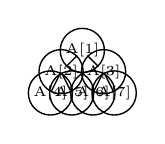
\begin{tikzpicture}[scale=0.45,
        level distance=0.6cm,
        level 1/.style={sibling distance=1.2cm},
        level 2/.style={sibling distance=0.6cm},
        every node/.style={circle,draw,inner sep=1pt,font=\tiny}]
        \node {A[1]}
            child {node {A[2]}
                child {node {A[4]}}
                child {node {A[5]}}
            }
            child {node {A[3]}
                child {node {A[6]}}
                child {node {A[7]}}
            };
    \end{tikzpicture}
    \caption*{\footnotesize Array indices in heap}
\end{figure}

\textbf{MAX-HEAPIFY Operation:}
\begin{enumerate}
    \item Compare root with children
    \item If child is larger, swap with largest child
    \item Recursively heapify affected subtree
\end{enumerate}

\begin{figure}[H]
    \centering
    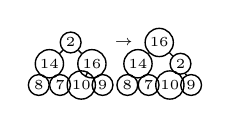
\begin{tikzpicture}[scale=0.45,
        level distance=0.6cm,
        level 1/.style={sibling distance=1.2cm},
        level 2/.style={sibling distance=0.6cm},
        every node/.style={circle,draw,inner sep=1pt,font=\tiny}]
        % Before MAX-HEAPIFY
        \node {2}
            child {node {14}
                child {node {8}}
                child {node {7}}
            }
            child {node {16}
                child {node {10}}
                child {node {9}}
            };
            
        % Arrow
        \node[draw=none] at (1.5,0) {$\rightarrow$};
        
        % After MAX-HEAPIFY
        \begin{scope}[xshift=2.5cm]
        \node {16}
            child {node {14}
                child {node {8}}
                child {node {7}}
            }
            child {node {2}
                child {node {10}}
                child {node {9}}
            };
        \end{scope}
    \end{tikzpicture}
    \caption*{\footnotesize MAX-HEAPIFY example}
\end{figure}

\textbf{BUILD-MAX-HEAP Operation:}
\begin{enumerate}
    \item Start from last non-leaf node ($\lfloor n/2 \rfloor$)
    \item Apply MAX-HEAPIFY to each node up to root
\end{enumerate}

\begin{figure}[H]
    \centering
    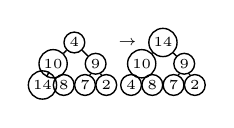
\begin{tikzpicture}[scale=0.45,
        level distance=0.6cm,
        level 1/.style={sibling distance=1.2cm},
        level 2/.style={sibling distance=0.6cm},
        every node/.style={circle,draw,inner sep=1pt,font=\tiny}]
        % Initial array as tree
        \node {4}
            child {node {10}
                child {node {14}}
                child {node {8}}
            }
            child {node {9}
                child {node {7}}
                child {node {2}}
            };
            
        % Arrow
        \node[draw=none] at (1.5,0) {$\rightarrow$};
        
        % After BUILD-MAX-HEAP
        \begin{scope}[xshift=2.5cm]
        \node {14}
            child {node {10}
                child {node {4}}
                child {node {8}}
            }
            child {node {9}
                child {node {7}}
                child {node {2}}
            };
        \end{scope}
    \end{tikzpicture}
    \caption*{\footnotesize BUILD-MAX-HEAP example}
\end{figure}

\textbf{HEAPSORT Operation:}
\begin{enumerate}
    \item BUILD-MAX-HEAP
    \item Repeatedly:
        \begin{itemize}[noitemsep,topsep=0pt]
            \item Swap root with last element
            \item Reduce heap size by 1
            \item MAX-HEAPIFY root
        \end{itemize}
\end{enumerate}

\clearpage
% Content from weeks 8-14
\clearpage
\section{\texorpdfstring{\underline{Graph Algorithms}}{Graph Algorithms}}
\subsection{Graph Representations}
\subsubsection{Graph Transpose}
\textbf{Problem Type:} Computing transpose $G^T$ of a directed graph $G=(V,E)$

\textbf{What to Look For:}
\begin{itemize}[noitemsep,leftmargin=*]
    \item Graph representation type (matrix/list)
    \item Direction of edges must be reversed
    \item Time complexity analysis required
\end{itemize}

\textbf{Key Definitions:}
\begin{itemize}[noitemsep,leftmargin=*]
    \item $G^T = (V,E^T)$ where $E^T = \{(v,u) \mid (u,v) \in E\}$
    \item $|V| = n$ (number of vertices)
    \item $|E|$ (number of edges)
\end{itemize}

\textbf{Solution for Adjacency Matrix:}
\begin{enumerate}[leftmargin=*,noitemsep]
    \item Given matrix $M_G$, create $M_G^T$ by swapping entries:
    \[ M = \begin{pmatrix}
        m_{11} & m_{12} & \cdots & m_{1n}\\
        m_{21} & m_{22} & \cdots & m_{2n}\\
        \vdots & \vdots & \ddots & \vdots\\
        m_{n1} & m_{n2} & \cdots & m_{nn}
    \end{pmatrix} \]
    
    \[ M^T = \begin{pmatrix}
        m_{11} & m_{21} & \cdots & m_{n1}\\
        m_{12} & m_{22} & \cdots & m_{n2}\\
        \vdots & \vdots & \ddots & \vdots\\
        m_{1n} & m_{2n} & \cdots & m_{nn}
    \end{pmatrix} \]

    \item Example:
    \[ M = \begin{pmatrix}1 & 2\\ 3 & 4\end{pmatrix}, 
       M^T = \begin{pmatrix}1 & 3\\ 2 & 4\end{pmatrix} \]
    
    \item Time Complexity: $\Theta(n^2)$
        \begin{itemize}[noitemsep]
            \item Must swap $n^2-n$ entries (excluding diagonal)
            \item Each swap is $O(1)$
        \end{itemize}
\end{enumerate}

\textbf{Solution for Adjacency List:}
\begin{enumerate}[leftmargin=*,noitemsep]
    \item Create empty adjacency lists for $G^T$: $O(n)$
    \item For each vertex $v$ in $G$:
        \begin{itemize}[noitemsep]
            \item For each edge $(v,w)$ in $v$'s adjacency list
            \item Add $v$ to $w$'s list in $G^T$
        \end{itemize}
    \item Time Complexity: $\Theta(|V| + |E|)$
        \begin{itemize}[noitemsep]
            \item Creating lists: $O(|V|)$
            \item Processing edges: $O(|E|)$
        \end{itemize}
\end{enumerate}

\textbf{Comparison:}
\begin{itemize}[noitemsep,leftmargin=*]
    \item Matrix: $\Theta(n^2)$ always
    \item List: $\Theta(|V| + |E|)$ which is better for sparse graphs
    \item List requires more complex implementation
\end{itemize}

\textbf{Common Mistakes to Avoid:}
\begin{itemize}[noitemsep,leftmargin=*]
    \item Don't forget self-loops (diagonal elements)
    \item Don't count diagonal elements in matrix swaps
    \item Remember to initialize all new lists in adjacency list solution
    \item Don't confuse $|V|$ and $|E|$ in complexity analysis
\end{itemize}

\FloatBarrier

\subsection{Shortest Paths}
\subsubsection{Dijkstra's Algorithm Limitations}
\textbf{Problem Type:} Counterexample for Dijkstra with negative weights

\textbf{What to Look For:}
\begin{itemize}[noitemsep,leftmargin=*]
    \item Directed graph with negative weights
    \item Minimal example showing algorithm failure
    \item Negative cycle demonstration
\end{itemize}

\textbf{Solution:}
\begin{enumerate}[leftmargin=*,noitemsep]
    \item Consider this directed graph:
    \begin{center}
    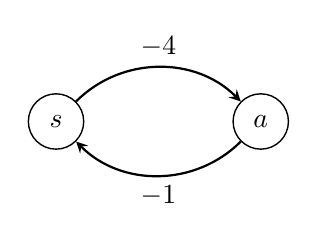
\begin{tikzpicture}[
        scale=1.3,
        vertex/.style={circle,draw,minimum size=20pt,inner sep=0pt}
    ]
        % Vertices
        \node[vertex] (s) at (0,0) {$s$};
        \node[vertex] (a) at (2,0) {$a$};
        
        % Curved edges
        \draw[thick,->,>=stealth] (s) to[bend left=45] node[above] {$-4$} (a);
        \draw[thick,->,>=stealth] (a) to[bend left=45] node[below] {$-1$} (s);
    \end{tikzpicture}
    \end{center}

    \item Why Dijkstra fails:
    \begin{itemize}[noitemsep]
        \item Initial distance to $a$: $-4$
        \item After one cycle: $-5$
        \item After two cycles: $-6$
        \item Continues to decrease indefinitely
    \end{itemize}
\end{enumerate}

\textbf{Key Properties:}
\begin{itemize}[noitemsep,leftmargin=*]
    \item Any negative cycle causes Dijkstra to fail
    \item Algorithm assumes:
        \begin{itemize}[noitemsep]
            \item Edge weights are non-negative
            \item Shortest paths exist (no negative cycles)
        \end{itemize}
    \item For negative weights, use Bellman-Ford instead
\end{itemize}

\textbf{Common Mistakes to Avoid:}
\begin{itemize}[noitemsep,leftmargin=*]
    \item Single negative edge isn't enough
    \item Example must have negative total cycle weight
\end{itemize}

\FloatBarrier


\clearpage
% Exercises
\clearpage

\section{Exercises}

\subsection{Exercise 1.1: Sorting Complexity}
\textbf{Problem:} A sorting method with “Big-Oh” complexity $O(n \log n)$ spends exactly 1 millisecond to sort 1,000 data items. Given this, estimate how long it will take to sort 1,000,000 items.

\vspace{0.5em}
\textbf{Solution Steps:}
\begin{enumerate}[leftmargin=*,noitemsep]
    \item Understand the Problem: You need to find out how long it will take to sort 1,000,000 items using the given complexity.
    \item Identify Known Values:
    \begin{itemize}
        \item $T(1,000) = 1ms$
        \item Complexity is $O(n \log n)$
    \end{itemize}
    \item Calculate Constant $c$:
    \begin{itemize}
        \item Formula: $T(n) = c \cdot n \log n$
        \item Use $T(1,000) = 1ms$ to find $c$:
        \[ c = \frac{1ms}{1,000 \log 1,000} \]
    \end{itemize}
    \item Calculate $T(1,000,000)$:
    \begin{itemize}
        \item Use the formula $T(n) = c \cdot n \log n$
        \item Substitute $n = 1,000,000$:
        \[ T(1,000,000) = c \cdot 1,000,000 \cdot \log 1,000,000 \]
    \end{itemize}
    \item Simplify the Expression:
    \begin{itemize}
        \item Calculate $\log 1,000,000$
        \item Multiply and simplify to find the time in seconds.
    \end{itemize}
\end{enumerate}

\textbf{Exam Note:} Remember that $O(n \log n)$ complexity means the time increases logarithmically with the size of the data.

\textbf{Hint:} To solve similar exercises, focus on understanding the relationship between the given complexity and the time it takes to process a certain amount of data. Use the formula $T(n) = c \cdot f(n)$ to calculate the constant $c$ and then use it to find the time for a different amount of data.

\subsection{Exercise 1.2: Quadratic Algorithm}
\textbf{Problem:} A quadratic algorithm with processing time $T(n) = cn^2$ spends 1ms for 100 items. Calculate the time for 5,000 items.

\vspace{0.5em}
\textbf{Solution Steps:}
\begin{enumerate}[leftmargin=*,noitemsep]
    \item Understand the Problem: You need to calculate the time for 5,000 items given the complexity.
    \item Identify Known Values:
    \begin{itemize}
        \item $T(100) = 1ms$
        \item Complexity is $O(n^2)$
    \end{itemize}
    \item Calculate Constant $c$:
    \begin{itemize}
        \item Formula: $T(n) = c \cdot n^2$
        \item Use $T(100) = 1ms$ to find $c$:
        \[ c = \frac{1ms}{100^2} \]
    \end{itemize}
    \item Calculate $T(5,000)$:
    \begin{itemize}
        \item Use the formula $T(n) = c \cdot n^2$
        \item Substitute $n = 5,000$:
        \[ T(5,000) = c \cdot (5,000)^2 \]
    \end{itemize}
    \item Simplify the Expression:
    \begin{itemize}
        \item Calculate $(5,000)^2$
        \item Multiply and simplify to find the time in milliseconds.
    \end{itemize}
\end{enumerate}

\textbf{Exam Note:} Quadratic complexity $O(n^2)$ means time increases with the square of the data size.

\textbf{Hint:} To solve similar exercises, focus on understanding the relationship between the given complexity and the time it takes to process a certain amount of data. Use the formula $T(n) = c \cdot f(n)$ to calculate the constant $c$ and then use it to find the time for a different amount of data.

\subsection{Exercise 1.3: Time Complexity}
\textbf{Problem:} Given $T(n) = c \cdot f(n)$, where $f(n) = n$ or $f(n) = n^3$, calculate the time for 100,000 items.

\vspace{0.5em}
\textbf{Solution Steps:}
\begin{enumerate}[leftmargin=*,noitemsep]
    \item Understand the Problem: You need to calculate the time for different functions $f(n)$.
    \item Identify Known Values:
    \begin{itemize}
        \item $T(1,000) = 10s$
        \item Functions $f(n) = n$ and $f(n) = n^3$
    \end{itemize}
    \item Calculate Constant $c$ for Each Function:
    \begin{itemize}
        \item Use $T(1,000) = 10s$ to find $c$ for each $f(n)$.
    \end{itemize}
    \item Calculate $T(100,000)$ for Each Function:
    \begin{itemize}
        \item For $f(n) = n$, compute $T(100,000)$.
        \item For $f(n) = n^3$, compute $T(100,000)$.
    \end{itemize}
    \item Simplify the Expressions:
    \begin{itemize}
        \item Calculate the necessary values and simplify.
    \end{itemize}
\end{enumerate}

\textbf{Exam Note:} Understand how different functions $f(n)$ affect time complexity.

\textbf{Hint:} To solve similar exercises, focus on understanding the relationship between the given complexity and the time it takes to process a certain amount of data. Use the formula $T(n) = c \cdot f(n)$ to calculate the constant $c$ and then use it to find the time for a different amount of data.

\subsection{Exercise 1.4: Dominant Terms}
\textbf{Problem:} Analyze expressions to find dominant terms and Big-Oh complexity.

\vspace{0.5em}
\textbf{Solution Steps:}
\begin{enumerate}[leftmargin=*,noitemsep]
    \item Understand the Problem: You need to identify the dominant term in each expression.
    \item Analyze Each Expression:
    \begin{itemize}
        \item Look for the term that grows fastest as $n$ increases.
        \item Example: For the expression $5n^2 + 3n \log n$, the term $5n^2$ grows faster than $3n \log n$.
    \end{itemize}
    \item Determine Big-Oh Notation:
    \begin{itemize}
        \item Use the dominant term to find the Big-Oh notation.
        \item Example: $5n^2 + 3n \log n$ is $O(n^2)$.
    \end{itemize}
    \item Practice with Examples:
    \begin{itemize}
        \item Expression: $n^3 + n^2 \log n$
        \item Dominant Term: $n^3$
        \item Big-Oh: $O(n^3)$
    \end{itemize}
\end{enumerate}

\textbf{Exam Note:} Focus on the term that grows fastest as $n$ increases.

\textbf{Hint:} To solve similar exercises, focus on identifying the dominant term in each expression. Use the properties of logarithms and powers of $n$ to analyze the relationships between terms and determine the Big-Oh notation.

\begin{table}[H]
    \centering
    \small
    \begin{tabularx}{\linewidth}{|>{\hsize=0.6\hsize}X|>{\hsize=0.4\hsize}X|}
    \hline
    \textbf{Expression} & \textbf{Big-Oh} \\
    \hline
    5 + 0.001$n^3$ + 0.025$n$ & $O(n^3)$ \\
    \hline
    500$n$ + 100$n^{1.5}$ + 50$n \log_{10} n$ & $O(n^{1.5})$ \\
    \hline
    0.3$n$ + 5$n^{1.5}$ + 2.5$n^{1.75}$ & $O(n^{1.75})$ \\
    \hline
    $n^2 \log_2 n$ + $n(n \log n)^2$ & $O(n^2 \log n)$ \\
    \hline
    $n \log_3 n$ + $n \log_2 n$ & $O(n \log n)$ \\
    \hline
    3$\log_8 n$ + $\log_2 \log_2 \log_2 n$ & $O(\log n)$ \\
    \hline
    100$n$ + 0.01$n^2$ & $O(n^2)$ \\
    \hline
    0.01$n$ + 100$n^2$ & $O(n^2)$ \\
    \hline
    2$n$ + $n^{0.5}$ + 0.5$n^{1.25}$ & $O(n^{1.25})$ \\
    \hline
    0.01$n \log_2 n$ + $n(\log_2 n)^2$ & $O(n(\log n)^2)$ \\
    \hline
    100$n \log_3 n$ + $n^3$ + 100$n$ & $O(n^3)$ \\
    \hline
    0.003$\log_4 n$ + $\log_2 \log_2 n$ & $O(\log n)$ \\
    \hline
    \end{tabularx}
    \caption{Dominant terms and Big-Oh notation for various expressions.}
\end{table}

\textbf{Exam Note:} Focus on the term that grows fastest as $n$ increases.

\textbf{Hint:} To solve similar exercises, focus on identifying the dominant term in each expression. Use the properties of logarithms and powers of $n$ to analyze the relationships between terms and determine the Big-Oh notation.

\subsection{Exercise 1.5: Big-Oh Notation}
\textbf{Problem:} Determine if statements about Big-Oh notation are true or false.

\vspace{0.5em}
\textbf{Solution Steps:}
\begin{enumerate}[leftmargin=*,noitemsep]
    \item Understand the Problem: You need to evaluate the truth of each statement about Big-Oh notation.
    \item Evaluate Each Statement:
    \begin{itemize}
        \item Rule of Sums: $O(f + g) = O(\max\{f, g\})$
        \item Rule of Products: $O(f \cdot g) = O(f) \cdot O(g)$
        \item Transitivity: If $g = O(f)$ and $h = O(g)$, then $h = O(f)$
    \end{itemize}
    \item Correct Any False Statements:
    \begin{itemize}
        \item If a statement is false, provide the correct formula.
        \item Example: If $O(f + g) = O(f) + O(g)$ is false, correct it to $O(f + g) = O(\max\{f, g\})$
    \end{itemize}
\end{enumerate}

\textbf{Exam Note:} Understand the properties of Big-Oh notation and be able to apply them to different scenarios.

\textbf{Hint:} To solve similar exercises, focus on understanding the properties of Big-Oh notation. Use the rules of sums, products, and transitivity to evaluate the truth of each statement.

\begin{table}[H]
    \centering
    \small
    \begin{tabularx}{\linewidth}{|>{\hsize=0.6\hsize}X|>{\hsize=0.4\hsize}X|}
    \hline
    \textbf{Statement} & \textbf{Evaluation} \\
    \hline
    Rule of sums: $O(f + g) = O(f) + O(g)$ & FALSE \\
    \hline
    Rule of products: $O(f \cdot g) = O(f) \cdot O(g)$ & TRUE \\
    \hline
    Transitivity: if $g = O(f)$ and $h = O(f)$ then $g = O(h)$ & FALSE \\
    \hline
    $5n + 8n^2 + 100n^3 = O(n^4)$ & TRUE \\
    \hline
    $5n + 8n^2 + 100n^3 = O(n^2 \log n)$ & FALSE \\
    \hline
    \end{tabularx}
    \caption{Evaluation of Big-Oh notation statements.}
\end{table}

\textbf{Exam Note:} Understand the properties of Big-Oh notation and be able to apply them to different scenarios.

\textbf{Hint:} To solve similar exercises, focus on understanding the properties of Big-Oh notation. Use the rules of sums, products, and transitivity to evaluate the truth of each statement.

\subsection{Exercise 1.6: Computational Complexity}
\textbf{Problem:} Analyze the complexity of a given algorithm.

\vspace{0.5em}
\textbf{Solution Steps:}
\begin{enumerate}[leftmargin=*,noitemsep]
    \item Understand the Problem: You need to break down the algorithm to find its complexity.
    \item Analyze Each Loop:
    \begin{itemize}
        \item Identify the number of iterations for each loop.
        \item Example: For a loop running from 1 to $n$, the complexity is $O(n)$.
    \end{itemize}
    \item Combine Results for Total Complexity:
    \begin{itemize}
        \item Multiply the complexities of nested loops.
        \item Example: A loop inside another loop, both running $n$ times, results in $O(n^2)$.
    \end{itemize}
    \item Simplify the Total Complexity:
    \begin{itemize}
        \item Combine terms to find the overall complexity.
        \item Example: If you have $O(n^2) + O(n)$, the dominant term is $O(n^2)$.
    \end{itemize}
\end{enumerate}

\textbf{Exam Note:} Pay close attention to nested loops and their impact on complexity. Practice breaking down algorithms into their basic components to understand their efficiency.

\textbf{Hint:} To solve similar exercises, focus on breaking down the algorithm into its basic components. Analyze each loop and combine the results to find the total complexity.

\FloatBarrier

\subsection{Exercise 2: Binary Search Tree Property}

\textbf{Problem:} Consider a binary search tree $T$ whose keys are distinct. Show that if the right subtree of a node $x$ in $T$ is empty and $x$ has a successor $y$, then $y$ is the lowest ancestor of $x$ whose left child is also an ancestor of $x$. (Recall that every node is its own ancestor.)

\textbf{Solution:} Let's prove this by contradiction:

\begin{enumerate}
    \item First, observe that since $x$ has no right subtree, its successor $y$ must be an ancestor of $x$.
        \begin{itemize}
            \item This is because in a BST, if $x$ had any right child, its successor would be in that subtree.
            \item Since there is no right subtree, we must go up the tree to find a larger value.
        \end{itemize}
    
    \item Assume for contradiction that there exists a node $z \neq y$ that is:
        \begin{itemize}
            \item The lowest ancestor of $x$ whose left child is an ancestor of $x$
            \item Different from $y$ (the successor of $x$)
        \end{itemize}
\end{enumerate}

\begin{figure}[H]
    \centering
    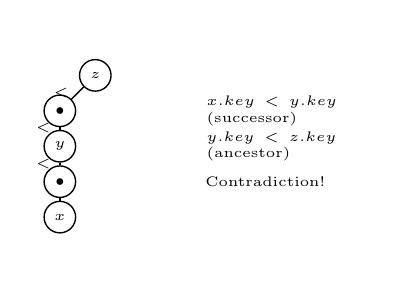
\begin{tikzpicture}[scale=0.45,
        level distance=1cm,
        level 1/.style={sibling distance=2cm},
        level 2/.style={sibling distance=1cm},
        every node/.style={circle,draw,inner sep=1pt,font=\tiny,minimum size=0.4cm}]
        
        % The tree showing contradiction
        \node (z) {$z$}
            child {
                node (leftz) {$\bullet$}
                child {
                    node (y) {$y$} 
                    child {
                        node (lefty) {$\bullet$}
                        child {
                            node (x) {$x$}
                        }
                        edge from parent node[left,draw=none,font=\tiny] {$<$}
                    }
                    edge from parent node[left,draw=none,font=\tiny] {$<$}
                }
                edge from parent node[left,draw=none,font=\tiny] {$<$}
            }
            child[missing];
            
        % Add explanatory text
        \node[draw=none,font=\tiny,text width=2cm,anchor=west] at (3,-1) 
            {$x.key < y.key$ (successor)};
        \node[draw=none,font=\tiny,text width=2cm,anchor=west] at (3,-2) 
            {$y.key < z.key$ (ancestor)};
        \node[draw=none,font=\tiny,text width=2cm,anchor=west] at (3,-3) 
            {Contradiction!};
    \end{tikzpicture}
    \caption*{\footnotesize Contradiction in BST property}
\end{figure}

This leads to a contradiction because:
\begin{itemize}
    \item Since $x$ is in the left subtree of $y$: $x.key < y.key$
    \item Since $z$ is an ancestor of $y$: $y.key < z.key$
    \item But $y$ is the successor of $x$, so there can't be any value $z.key$ between $x.key$ and $y.key$
    \item Therefore, $z$ must be $y$
\end{itemize}

Thus, $y$ (the successor of $x$) must be the lowest ancestor of $x$ whose left child is also an ancestor of $x$.

\subsection{Exercise 2.1: Heap Structure}
\textbf{Problem:} Viewing a heap as a tree, we define the height of a node in a heap to be the number of edges on the longest simple downward path from the node to a leaf, and we define the height of the heap to be the height of its root. What are the minimum and maximum numbers of elements in a heap of height $h$?

\vspace{0.5em}
\textbf{Solution:} From the previous exercise (in particular its solution) we have seen that

\[ 2^h \leq n \leq 2^{h+1} - 1 \]

where $h$ is the height of the complete binary tree. By taking the logarithm $\lg$ in base 2 at each term of the above sequence of inequalities, since $\lg$ is a monotone increasing function we have

\[ h \leq \ln n \leq \ln(2^{h+1} - 1) \]

Now it is enough to note that

\[ h = \ln 2^h \leq \ln n \leq \ln(2^{h+1} - 1) < h + 1 \]

Thus we have

\[ h = \lfloor h \rfloor \leq \lfloor \ln n \rfloor \leq \lfloor \ln(2^{h+1} - 1) \rfloor = h \]

\begin{figure}[H]
    \centering
    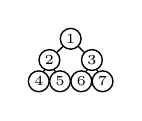
\begin{tikzpicture}[scale=0.45,
        level distance=0.6cm,
        level 1/.style={sibling distance=1.2cm},
        level 2/.style={sibling distance=0.6cm},
        every node/.style={circle,draw,inner sep=1pt,font=\tiny}]
        \node {1}
            child {node {2}
                child {node {4}}
                child {node {5}}
            }
            child {node {3}
                child {node {6}}
                child {node {7}}
            };
    \end{tikzpicture}
    \caption*{\footnotesize Simple Binary Tree Representing a Heap}
\end{figure}

\textbf{Hint:} To solve similar exercises, focus on understanding the structure of heaps and binary trees. Use the properties of logarithms and powers of 2 to analyze the relationships between nodes and height.

\subsection{Exercise 2.2: Heap Height}
\textbf{Problem:} Show that an $n$-element heap has height $\lfloor \lg n \rfloor$. (Where $\lg(\cdot)$ denotes logarithm in base 2).

\vspace{0.5em}
\textbf{Solution:} From the previous exercise (in particular its solution) we have seen that

\[ 2^h \leq n \leq 2^{h+1} - 1 \]

where $h$ is the height of the complete binary tree. By taking the logarithm $\lg$ in base 2 at each term of the above sequence of inequalities, since $\lg$ is a monotone increasing function we have

\[ h \leq \ln n \leq \ln(2^{h+1} - 1) \]

Now it is enough to note that

\[ h = \ln 2^h \leq \ln n \leq \ln(2^{h+1} - 1) < h + 1 \]

Thus we have

\[ h = \lfloor h \rfloor \leq \lfloor \ln n \rfloor \leq \lfloor \ln(2^{h+1} - 1) \rfloor = h \]

\textbf{Hint:} To solve similar exercises, focus on understanding the structure of heaps and binary trees. Use the properties of logarithms and powers of 2 to analyze the relationships between nodes and height.

\subsection{Exercise 2.4: Recursive Algorithm Running Time}
\textbf{Problem:} We consider the running time of a recursive algorithm $y(n)$. Suppose that $y(n)$ verifies the following:

1. \[
\begin{cases}
    y(1) = 0 \\
    y(n) = y\left(\frac{n}{2}\right) + 1 & n \geq 1
\end{cases}
\]
If possible, calculate the running time.

2. \[
\begin{cases}
    y(1) = 0 \\
    y(n) = 3y\left(\frac{n}{4}\right) + n^2 \log_2 n & n \geq 1
\end{cases}
\]
If possible, calculate the running time.

3. \[
\begin{cases}
    y(1) = 0 \\
    y(n) = 5y\left(\frac{n}{3}\right) + \log_2 n & n \geq 1
\end{cases}
\]
If possible, calculate the running time.

\vspace{0.5em}
\textbf{Solution:} Using the Master Theorem:

1. We have $a = 1$, $b = 2$, and $f(n) = 1$. Since $n^{\log_b a} = n^0 = 1$, we have $f(n) = \Theta(1)$. Thus we are in case II of the Master Theorem. So $T(n) = \Theta(\ln n)$.

2. We have $a = 3$, $b = 4$, and $f(n) = n^2 \log_2 n$. Since $n^{\log_b a} = n^{\log_4 3}$, we have $f(n) = \Omega(n^{\log_4 3 + \epsilon})$ for some $\epsilon > 0$. Therefore, for the Master Theorem (case 3), we have $T(n) = \Theta(n^2 \ln n)$.

3. We have $a = 5$, $b = 3$, and $f(n) = \log_2 n$. Since $n^{\log_b a} = n^{\log_3 5} > n$, we have $f(n) = O(n^{\log_3 5 - \epsilon})$ for some $\epsilon > 0$. Therefore, we are in case 1 of the Master Theorem, and so $T(n) = \Theta(n^{\log_3 5})$. 

\textbf{Conclusion:} To apply the Master Theorem, follow these steps:

1. Identify the parameters $a$, $b$, and $f(n)$ from the recurrence relation.
2. Calculate $n^{\log_b a}$ to compare with $f(n)$.
3. Determine which case of the Master Theorem applies:
   - \textbf{Case 1:} If $f(n)$ grows slower than $n^{\log_b a}$, then $T(n) = \Theta(n^{\log_b a})$.
   - \textbf{Case 2:} If $f(n)$ grows at the same rate as $n^{\log_b a}$, then $T(n) = \Theta(n^{\log_b a} \log n)$.
   - \textbf{Case 3:} If $f(n)$ grows faster than $n^{\log_b a}$, then check the regularity condition. If it holds, $T(n) = \Theta(f(n))$.

This approach helps in determining the asymptotic behavior of recursive algorithms efficiently.

\textbf{Hint:} To solve similar exercises, identify the parameters $a$, $b$, and $f(n)$ in the recurrence relation, and apply the Master Theorem to determine the running time.

\subsection{Exercise 3.1: HEAPSORT Operations}
\textbf{Problem:} Using the figure in slide 25 of the slide of week 2 as a model, illustrate the operations of HEAPSORT on the array

\[ A = \{5, 13, 2, 25, 7, 17, 20, 8, 4\} \]

\vspace{0.5em}
\textbf{Solution:} Let's break down the HEAPSORT process into detailed steps:

1. \textbf{Build Max-Heap (BUILD-MAX-HEAP)}:
   \begin{itemize}
      \item Start with the array as a binary tree (parent at $i$, children at $2i$ and $2i+1$)
      \item For each non-leaf node from $\lfloor n/2 \rfloor$ down to 1:
         \begin{itemize}
            \item Call MAX-HEAPIFY on that node
            \item This ensures the subtree rooted at each node satisfies max-heap property
         \end{itemize}
   \end{itemize}

2. \textbf{Extract and Sort (HEAPSORT)}:
   \begin{itemize}
      \item For $i$ from $n$ down to 2:
         \begin{itemize}
            \item Swap $A[1]$ (root) with $A[i]$ (last element)
            \item Reduce heap size by 1
            \item Call MAX-HEAPIFY on root (1) to maintain max-heap property
         \end{itemize}
   \end{itemize}

\textbf{Detailed Process for Our Array}:
\begin{enumerate}[label=\arabic*.]
    \item Initial array: $\{5, 13, 2, 25, 7, 17, 20, 8, 4\}$
    \item BUILD-MAX-HEAP:
       \begin{itemize}
          \item Start from last non-leaf node ($\lfloor 9/2 \rfloor = 4$)
          \item Apply MAX-HEAPIFY at each level up to root
          \item Results in max-heap with 25 at root
       \end{itemize}
    \item HEAPSORT Process:
       \begin{itemize}
          \item Swap 25 with last element, heapify remaining
          \item Swap new max with second-to-last, heapify
          \item Continue until all elements processed
       \end{itemize}
    \item Final sorted array: $\{2, 4, 5, 7, 8, 13, 17, 20, 25\}$
\end{enumerate}

\textbf{Key Operations}:
\begin{itemize}
    \item MAX-HEAPIFY($A,i$): Ensures subtree at index $i$ maintains max-heap property
    \item BUILD-MAX-HEAP($A$): Converts array into max-heap
    \item HEAPSORT($A$): Repeatedly extracts maximum and rebuilds heap
\end{itemize}

\begin{figure}[H]
    \centering
    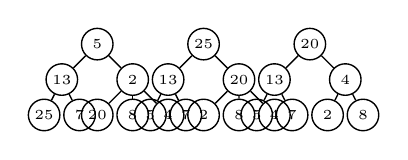
\begin{tikzpicture}[scale=0.45,
        level distance=1cm,
        level 1/.style={sibling distance=2cm},
        level 2/.style={sibling distance=1cm},
        level 3/.style={sibling distance=0.8cm},
        every node/.style={circle,draw,inner sep=1pt,font=\tiny,minimum size=0.4cm}]
        
        % Initial tree
        \node {5}
            child {node {13}
                child {node {25}}
                child {node {7}}
            }
            child {node {2}
                child {node {20}}
                child {node {8}}
                child {node {4}}
            };
            
        % After BUILD-MAX-HEAP
        \begin{scope}[xshift=3cm]
        \node {25}
            child {node {13}
                child {node {5}}
                child {node {7}}
            }
            child {node {20}
                child {node {2}}
                child {node {8}}
                child {node {4}}
            };
        \end{scope}
        
        % After first extraction
        \begin{scope}[xshift=6cm]
        \node {20}
            child {node {13}
                child {node {5}}
                child {node {7}}
            }
            child {node {4}
                child {node {2}}
                child {node {8}}
            };
        \end{scope}
    \end{tikzpicture}
    \caption*{\footnotesize HEAPSORT steps: Initial $\rightarrow$ BUILD-MAX-HEAP $\rightarrow$ First extraction}
\end{figure}

\textbf{Note:} The process continues similarly until all elements are sorted. At each step:
\begin{itemize}
    \item The largest element moves to the root
    \item We swap it with the last element of the current heap
    \item We reduce the heap size and MAX-HEAPIFY the root
\end{itemize}

\textbf{Hint:} To solve similar exercises:
\begin{enumerate}
    \item Draw the initial array as a complete binary tree
    \item Apply BUILD-MAX-HEAP by working bottom-up
    \item For each HEAPSORT step:
       \begin{itemize}
          \item Draw the current heap state
          \item Show the swap operation
          \item Show the heapified result
       \end{itemize}
    \item Keep track of the sorted portion at the end of the array
\end{enumerate}

\subsection{Exercise 3.2: Tree Predecessor}
\textbf{Problem:} Write the TREE-PREDECESSOR procedure.

\textbf{Solution:} To obtain TREE-PREDECESSOR(x) procedure, we replace in TREE-SUCCESSOR(x) ``left'' instead of ``right'' and ``MAXIMUM'' instead of ``MINIMUM''.

\begin{algorithm}[H]
\begin{algorithmic}[1]
\Procedure{Tree-Predecessor}{$x$}
    \If{$x.right \neq \text{NIL}$}
        \State \Return Tree-Maximum($x.left$)
    \EndIf
    \State $y \gets x.p$
    \While{$y \neq \text{NIL}$ \textbf{and} $x = y.left$}
        \State $x \gets y$
        \State $y \gets y.p$
    \EndWhile
    \State \Return $y$
\EndProcedure
\end{algorithmic}
\end{algorithm}

\begin{figure}[H]
    \centering
    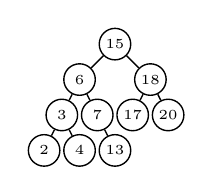
\begin{tikzpicture}[scale=0.45,
        level distance=1cm,
        level 1/.style={sibling distance=2cm},
        level 2/.style={sibling distance=1cm},
        every node/.style={circle,draw,inner sep=1pt,font=\tiny,minimum size=0.4cm}]
        
        % Example tree for predecessor
        \node {15}
            child {
                node {6}
                child {
                    node {3}
                    child {node {2}}
                    child {node {4}}
                }
                child {
                    node {7}
                    child[missing]
                    child {node {13}}
                }
            }
            child {
                node {18}
                child {node {17}}
                child {node {20}}
            };
    \end{tikzpicture}
    \caption*{\footnotesize Example: Predecessor of 15 is 13 (maximum in left subtree)}
\end{figure}

\textbf{Explanation:}
\begin{itemize}
    \item Case 1: If $x$ has a left subtree, the predecessor is the maximum element in that subtree
    \item Case 2: If no left subtree exists, we go up the tree until we find a node that is a right child
    \item The predecessor's key is the largest key in the tree smaller than $x.key$
\end{itemize}

\subsection{Exercise 3.4: Binary Search Tree Insertion}
\textbf{Problem:} Let $T$ be a Binary Search Tree. Prove that it always possible to insert a node $z$ as a leaf of the tree $T$ with $z.key = r$.

\textbf{Solution:} This is a straightforward property of Binary Search Trees. We prove this by induction on the height of the tree.

\begin{itemize}
\item \textbf{Base case} ($h = 0$):
    \begin{itemize}
        \item Tree consists only of root node $x$
        \item If $r \leq x.key$: place $z$ as left child of $x$
        \item If $r > x.key$: place $z$ as right child of $x$
    \end{itemize}

\item \textbf{Inductive step:}
    \begin{itemize}
        \item Assume the statement is true for trees of height $h-1$
        \item For a tree of height $h$ with root $x$:
        \begin{itemize}
            \item If $r \leq x.key$: insert in left subtree
            \item If $r > x.key$: insert in right subtree
        \end{itemize}
        \item By inductive hypothesis, we can insert in the chosen subtree (height $h-1$)
    \end{itemize}
\end{itemize}

\begin{figure}[H]
    \centering
    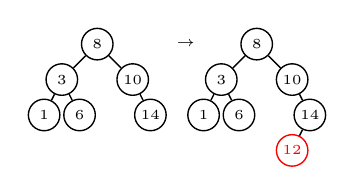
\begin{tikzpicture}[scale=0.45,
        level distance=1cm,
        level 1/.style={sibling distance=2cm},
        level 2/.style={sibling distance=1cm},
        every node/.style={circle,draw,inner sep=1pt,font=\tiny,minimum size=0.4cm}]
        
        % Before insertion
        \node {8}
            child {
                node {3}
                child {node {1}}
                child {node {6}}
            }
            child {
                node {10}
                child[missing]
                child {node {14}}
            };
            
        % Arrow
        \node[draw=none] at (2.5,0) {$\rightarrow$};
        
        % After insertion of 12
        \begin{scope}[xshift=4.5cm]
        \node {8}
            child {
                node {3}
                child {node {1}}
                child {node {6}}
            }
            child {
                node {10}
                child[missing]
                child {
                    node {14}
                    child {node[red] {12}}
                    child[missing]
                }
            };
        \end{scope}
    \end{tikzpicture}
    \caption*{\footnotesize Example: Inserting node with key=12 (shown in red)}
\end{figure}

\textbf{Key Points:}
\begin{itemize}
    \item The BST property ensures we can always find a valid leaf position
    \item At each step, we reduce the problem to a smaller subtree
    \item The process terminates when we reach a NULL child pointer
    \item Insertion maintains the BST property
\end{itemize}

\subsection{Exercise 3.2: Tree Predecessor}
\textbf{Problem:} Write the TREE-PREDECESSOR procedure.

\textbf{Solution:} To obtain TREE-PREDECESSOR(x) procedure, we replace in TREE-SUCCESSOR(x) ``left'' instead of ``right'' and ``MAXIMUM'' instead of ``MINIMUM''.

\begin{algorithm}[H]
\begin{algorithmic}[1]
\Procedure{Tree-Predecessor}{$x$}
    \If{$x.right \neq \text{NIL}$}
        \State \Return Tree-Maximum($x.left$)
    \EndIf
    \State $y \gets x.p$
    \While{$y \neq \text{NIL}$ \textbf{and} $x = y.left$}
        \State $x \gets y$
        \State $y \gets y.p$
    \EndWhile
    \State \Return $y$
\EndProcedure
\end{algorithmic}
\end{algorithm}

\begin{figure}[H]
    \centering
    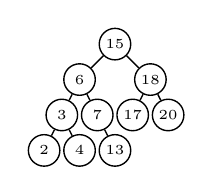
\begin{tikzpicture}[scale=0.45,
        level distance=1cm,
        level 1/.style={sibling distance=2cm},
        level 2/.style={sibling distance=1cm},
        every node/.style={circle,draw,inner sep=1pt,font=\tiny,minimum size=0.4cm}]
        
        % Example tree for predecessor
        \node {15}
            child {
                node {6}
                child {
                    node {3}
                    child {node {2}}
                    child {node {4}}
                }
                child {
                    node {7}
                    child[missing]
                    child {node {13}}
                }
            }
            child {
                node {18}
                child {node {17}}
                child {node {20}}
            };
    \end{tikzpicture}
    \caption*{\footnotesize Example: Predecessor of 15 is 13 (maximum in left subtree)}
\end{figure}

\textbf{Explanation:}
\begin{itemize}
    \item Case 1: If $x$ has a left subtree, the predecessor is the maximum element in that subtree
    \item Case 2: If no left subtree exists, we go up the tree until we find a node that is a right child
    \item The predecessor's key is the largest key in the tree smaller than $x.key$
\end{itemize}

\subsection{Exercise 3.4: Binary Search Tree Insertion}
\textbf{Problem:} Let $T$ be a Binary Search Tree. Prove that it always possible to insert a node $z$ as a leaf of the tree $T$ with $z.key = r$.

\textbf{Solution:} This is a straightforward property of Binary Search Trees. We prove this by induction on the height of the tree.

\begin{proof}
\begin{itemize}
\item \textbf{Base case} ($h = 0$):
    \begin{itemize}
        \item Tree consists only of root node $x$
        \item If $r \leq x.key$: place $z$ as left child of $x$
        \item If $r > x.key$: place $z$ as right child of $x$
    \end{itemize}

\item \textbf{Inductive step:}
    \begin{itemize}
        \item Assume the statement is true for trees of height $h-1$
        \item For a tree of height $h$ with root $x$:
        \begin{itemize}
            \item If $r \leq x.key$: insert in left subtree
            \item If $r > x.key$: insert in right subtree
        \end{itemize}
        \item By inductive hypothesis, we can insert in the chosen subtree (height $h-1$)
    \end{itemize}
\end{itemize}
\end{proof}

\begin{figure}[H]
    \centering
    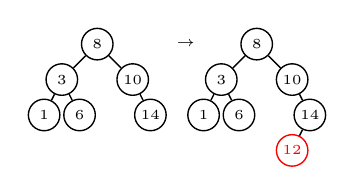
\begin{tikzpicture}[scale=0.45,
        level distance=1cm,
        level 1/.style={sibling distance=2cm},
        level 2/.style={sibling distance=1cm},
        every node/.style={circle,draw,inner sep=1pt,font=\tiny,minimum size=0.4cm}]
        
        % Before insertion
        \node {8}
            child {
                node {3}
                child {node {1}}
                child {node {6}}
            }
            child {
                node {10}
                child[missing]
                child {node {14}}
            };
            
        % Arrow
        \node[draw=none] at (2.5,0) {$\rightarrow$};
        
        % After insertion of 12
        \begin{scope}[xshift=4.5cm]
        \node {8}
            child {
                node {3}
                child {node {1}}
                child {node {6}}
            }
            child {
                node {10}
                child[missing]
                child {
                    node {14}
                    child {node[red] {12}}
                    child[missing]
                }
            };
        \end{scope}
    \end{tikzpicture}
    \caption*{\footnotesize Example: Inserting node with key=12 (shown in red)}
\end{figure}

\textbf{Key Points:}
\begin{itemize}
    \item The BST property ensures we can always find a valid leaf position
    \item At each step, we reduce the problem to a smaller subtree
    \item The process terminates when we reach a NULL child pointer
    \item Insertion maintains the BST property
\end{itemize}

\subsection{Exercise 3.5: Binary Search Tree Deletion}
\textbf{Problem:} Let $T$ be a Binary Search Tree given in the figure below. Give the output tree after the call of TREE-DELETE$(T, z)$ where $z$ is the node with key 41.

\begin{figure}[H]
    \centering
    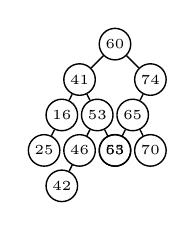
\begin{tikzpicture}[scale=0.45,
        level distance=1cm,
        level 1/.style={sibling distance=2cm},
        level 2/.style={sibling distance=1cm},
        every node/.style={circle,draw,inner sep=1pt,font=\tiny,minimum size=0.4cm}]
        
        % Initial tree
        \node {60}
            child {
                node {41}
                child {
                    node {16}
                    child {node {25}}
                    child[missing]
                }
                child {
                    node {53}
                    child {
                        node {46}
                        child {node {42}}
                        child[missing]
                    }
                    child {node {55}}
                }
            }
            child {
                node {74}
                child {
                    node {65}
                    child {node {63}}
                    child {node {70}}
                }
                child[missing]
            };
    \end{tikzpicture}
    \caption*{\footnotesize Initial Binary Search Tree with node 41 to be deleted}
\end{figure}

\textbf{Algorithm: TREE-DELETE$(T,z)$}
\begin{algorithm}[H]
\begin{algorithmic}[1]
\Procedure{Tree-Delete}{$T,z$}
    \If{$z.left = \text{NIL}$}
        \State \textsc{Transplant}$(T,z,z.right)$
    \ElsIf{$z.right = \text{NIL}$}
        \State \textsc{Transplant}$(T,z,z.left)$
    \Else
        \State $y \gets \text{Tree-Minimum}(z.right)$
        \If{$y.p \neq z$}
            \State \textsc{Transplant}$(T,y,y.right)$
            \State $y.right \gets z.right$
            \State $y.right.p \gets y$
        \EndIf
        \State \textsc{Transplant}$(T,z,y)$
        \State $y.left \gets z.left$
        \State $y.left.p \gets y$
    \EndIf
\EndProcedure
\end{algorithmic}
\end{algorithm}

\textbf{Solution:} Let's solve this step by step following the TREE-DELETE algorithm:

\begin{enumerate}
    \item \textbf{Analyze the node to be deleted (41):}
        \begin{itemize}
            \item Node 41 has two children: 16 (left) and 53 (right)
            \item Since it has two children, we fall into the third case (lines 7-15)
            \item We need to find its successor to replace it
        \end{itemize}
    
    \item \textbf{Find the successor of 41 (lines 7):}
        \begin{itemize}
            \item Call TREE-MINIMUM$(z.right)$ to find successor
            \item Right subtree starts at node 53
            \item Follow left pointers: 53 → 46 → 42
            \item Node 42 has no left child, so it's the successor
        \end{itemize}
    
    \item \textbf{Handle successor's position (lines 8-11):}
        \begin{itemize}
            \item Check if successor (42) is not a direct child of 41
            \item Since 42 is not direct child (it's grandchild), we:
                \begin{itemize}
                    \item Replace 42 with its right child (NIL in this case)
                    \item Make 42 point to 41's right child (53)
                    \item Make 53's parent point to 42
                \end{itemize}
        \end{itemize}

    \item \textbf{Complete the replacement (lines 12-14):}
        \begin{itemize}
            \item Replace 41 with 42 using TRANSPLANT
            \item Make 42 point to 41's left child (16)
            \item Make 16's parent point to 42
        \end{itemize}
\end{enumerate}

\begin{figure}[H]
    \centering
    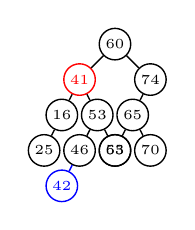
\begin{tikzpicture}[scale=0.45,
        level distance=1cm,
        level 1/.style={sibling distance=2cm},
        level 2/.style={sibling distance=1cm},
        every node/.style={circle,draw,inner sep=1pt,font=\tiny,minimum size=0.4cm}]
        
        % Intermediate step - finding successor
        \node {60}
            child {
                node[red] {41}
                child {
                    node {16}
                    child {node {25}}
                    child[missing]
                }
                child {
                    node {53}
                    child {
                        node {46}
                        child[blue] {node {42}}
                        child[missing]
                    }
                    child {node {55}}
                }
            }
            child {
                node {74}
                child {
                    node {65}
                    child {node {63}}
                    child {node {70}}
                }
                child[missing]
            };
    \end{tikzpicture}
    \caption*{\footnotesize Finding successor: Node to delete (41) in red, successor (42) in blue}
\end{figure}

\begin{figure}[H]
    \centering
    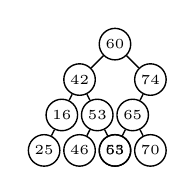
\begin{tikzpicture}[scale=0.45,
        level distance=1cm,
        level 1/.style={sibling distance=2cm},
        level 2/.style={sibling distance=1cm},
        every node/.style={circle,draw,inner sep=1pt,font=\tiny,minimum size=0.4cm}]
        
        % Final tree after deletion
        \node {60}
            child {
                node {42}
                child {
                    node {16}
                    child {node {25}}
                    child[missing]
                }
                child {
                    node {53}
                    child {
                        node {46}
                    }
                    child {node {55}}
                }
            }
            child {
                node {74}
                child {
                    node {65}
                    child {node {63}}
                    child {node {70}}
                }
                child[missing]
            };
    \end{tikzpicture}
    \caption*{\footnotesize Final Binary Search Tree after deleting node 41}
\end{figure}

\textbf{Key Points for Tree Deletion:}
\begin{itemize}
    \item There are three cases when deleting a node:
        \begin{enumerate}
            \item Node has no children (leaf node):
                \begin{itemize}
                    \item Simply remove it by setting parent's pointer to NIL
                    \item Example: Deleting a leaf like node 25
                \end{itemize}
            
            \item Node has one child:
                \begin{itemize}
                    \item Replace node with its only child
                    \item Update parent pointers
                    \item Example: If node 16 had only child 25
                \end{itemize}
            
            \item Node has two children:
                \begin{itemize}
                    \item Find successor (smallest value in right subtree)
                    \item Replace node with successor
                    \item Handle successor's original position
                    \item Example: Node 41 in our case
                \end{itemize}
        \end{enumerate}
    
    \item Finding the successor (TREE-MINIMUM):
        \begin{itemize}
            \item Start at node's right child
            \item Keep following left pointers until NIL
            \item Last node found is successor
            \item Important: Successor never has a left child
        \end{itemize}
    
    \item TRANSPLANT operation:
        \begin{itemize}
            \item Used to replace one subtree with another
            \item Updates parent pointers correctly
            \item Handles special case of root node
            \item Does not handle child pointers of moved nodes
        \end{itemize}
\end{itemize}

\textbf{Verification:} After deletion:
\begin{itemize}
    \item Node 42 maintains BST property:
        \begin{itemize}
            \item Left subtree (16, 25) contains values < 42
            \item Right subtree (53, 46, 55) contains values > 42
        \end{itemize}
    \item Tree structure remains valid:
        \begin{itemize}
            \item All parent-child pointers are correct
            \item No nodes were lost or duplicated
        \end{itemize}
    \item BST invariants are preserved:
        \begin{itemize}
            \item For every node: left subtree values < node key < right subtree values
            \item Tree remains connected
            \item No cycles are created
        \end{itemize}
\end{itemize}

\subsection{Exercise 4.1: Quicksort Partitioning Worst Case}
\textbf{Problem:} Prove that the worst case in Partitioning Algorithm (for Quicksort) has running time $\Theta(n^2)$, where $n$ is the cardinality of the set of elements in the partitioning.

\textbf{Solution:} We provide both an intuitive proof and a formal proof by induction.

\textbf{Part 1: Intuitive Proof}
\begin{enumerate}[leftmargin=*,noitemsep]
    \item \textbf{Worst Case Scenario:}
    \begin{itemize}[noitemsep]
        \item At each step, we get maximally unbalanced partitions:
        \item A $k-1$ element array and an empty array
        \item This happens when pivot is always smallest/largest element
    \end{itemize}

    \item \textbf{Recurrence Relation:}
    Let $T(n)$ be the running time of Quicksort with Partition:
    \begin{itemize}[noitemsep]
        \item Splitting time is linear: $\Theta(k)$ for array of size $k$
        \item Base case: $T(0)$ is constant, so $T(0) = \Theta(1)$
        \item For size $k$: $T(k) = T(k-1) + T(0) + \Theta(k)$
        \item Simplifies to: $T(k) = T(k-1) + \Theta(k)$
    \end{itemize}

    \item \textbf{Solving the Recurrence:}
    \begin{align*}
        T(n) &= T(n-1) + \Theta(n) \\
        &= T(n-2) + \Theta(n-1) + \Theta(n) \\
        &= T(n-3) + \Theta(n-2) + \Theta(n-1) + \Theta(n) \\
        &\vdots \\
        &= T(0) + \sum_{i=1}^n \Theta(i)
    \end{align*}

    \item \textbf{Final Step:}
    \begin{itemize}[noitemsep]
        \item Sum is arithmetic series: $\sum_{i=1}^n i$
        \item Using identity: $\sum_{i=1}^n i = \frac{n(n+1)}{2}$
        \item Therefore: $T(n) = \Theta(n^2)$
    \end{itemize}
\end{enumerate}

\textbf{Part 2: Formal Proof by Induction}
\begin{enumerate}[leftmargin=*,noitemsep]
    \item \textbf{Claim:} $T(n) = \Theta(n^2)$ for worst-case running time
    
    \item \textbf{Precise Statement:}
    \begin{itemize}[noitemsep]
        \item For all $0 < m < n$: $T(m) = \Theta(m^2)$
        \item This means $\exists c_1,d_1 > 0: c_1m^2 \leq T(m) \leq d_1m^2$
        \item Partition time $P(m) = \Theta(m)$, so $\exists c_2,d_2 > 0: c_2m \leq P(m) + T(0) \leq d_2m$
    \end{itemize}

    \item \textbf{Constants:}
    \begin{itemize}[noitemsep]
        \item Let $c = \min\{c_1,c_2\}$ and $d = \max\{d_1,d_2,1\}$
        \item Then for all $m \geq n-1$: $cm^2 \leq T(m) \leq dm^2$
        \item And for all $m \geq n$: $2cm \leq T(0) + P(m) \leq dm$
    \end{itemize}

    \item \textbf{Inductive Step:}
    \begin{align*}
        T(n) &= T(n-1) + T(0) + P(n) \\
        c(n-1)^2 + 2cn &\leq cn^2 - 2cn + 1 + 2cn = cn^2 + 1 \\
        d(n-1)^2 + dn &\leq dn^2 - dn + 1 \leq dn^2
    \end{align*}

    Therefore: $cn^2 < T(n) \leq dn^2$, proving $T(n) = \Theta(n^2)$
\end{enumerate}

\textbf{Key Insights:}
\begin{itemize}[noitemsep]
    \item The worst case occurs with extremely unbalanced partitions
    \item Each partition step costs linear time
    \item The cumulative effect leads to quadratic runtime
    \item Both intuitive and formal proofs confirm $\Theta(n^2)$ complexity
\end{itemize}

\subsection{Exercise 4.2: COUNTING-SORT Algorithm}
\textbf{Problem:} We apply COUNTING-SORT with the input vector $A = (5,6,5,3,3,7,4,4,4,5,3,8,8)$. Let $C$ and $B$ be the arrays mentioned in the pseudocode of COUNTING-SORT. Answer the following questions:

\begin{enumerate}[leftmargin=*,noitemsep]
    \item What is $C[7]$ after the for loop at lines 7-8 of the pseudocode?
    \item What is $B[13]$ after the first cycle at line 10?
    \item What is $C[8]$ after the first cycle?
\end{enumerate}

\textbf{Solution:} Let's solve this step by step following the COUNTING-SORT algorithm.

\textbf{1. Algorithm Overview:}
\begin{itemize}[noitemsep]
    \item Input array $A = (5,6,5,3,3,7,4,4,4,5,3,8,8)$ with $k=8$ (max value)
    \item Array $C[0..k]$ is used for counting and cumulative sums
    \item Array $B[1..n]$ will store the sorted output
\end{itemize}

\textbf{2. Step-by-Step Execution:}
\begin{enumerate}[leftmargin=*,noitemsep]
    \item \textbf{Initialize array $C$:}
    \begin{itemize}[noitemsep]
        \item Create $C[0..8]$ initialized to zeros
        \item $C = [0,0,0,0,0,0,0,0,0]$
    \end{itemize}

    \item \textbf{Count elements (lines 3-4):}
    \begin{itemize}[noitemsep]
        \item Count occurrences of each value in $A$
        \item After this step: $C = [0,0,0,3,3,3,1,1,2]$
        \item Meaning: three 3s, three 4s, three 5s, one 6, one 7, two 8s
    \end{itemize}

    \item \textbf{Compute cumulative sums (lines 5-6):}
    \begin{itemize}[noitemsep]
        \item Transform $C$ into cumulative counts
        \item $C = [0,0,0,3,6,9,10,11,13]$
        \item Therefore, $C[7] = 11$ (\textbf{Answer to Question 1})
    \end{itemize}

    \item \textbf{Build sorted array (lines 7-8):}
    \begin{itemize}[noitemsep]
        \item Process $A$ from right to left
        \item Place elements in $B$ based on $C$ values
        \item After first cycle (processing last element 8):
            \begin{itemize}[noitemsep]
                \item $B[13] = 8$ (\textbf{Answer to Question 2})
                \item $C[8]$ is decremented to 12 (\textbf{Answer to Question 3})
            \end{itemize}
        \item Final sorted array: $B = [3,3,3,4,4,4,5,5,5,6,7,8,8]$
    \end{itemize}
\end{enumerate}

\textbf{Key Insights:}
\begin{itemize}[noitemsep]
    \item The cumulative sum array $C$ helps maintain stability by tracking positions
    \item Processing from right to left ensures stability
    \item $C[i]$ represents the position after which the next element $i$ should be placed
    \item Each placement decrements the corresponding counter in $C$
\end{itemize}

\textbf{Final Answers:}
\begin{enumerate}[noitemsep]
    \item $C[7] = 11$
    \item $B[13] = 8$
    \item $C[8] = 12$
\end{enumerate}

\subsection{Exercise 5.1: BUILDKDTREE Algorithm}
\textbf{Problem:} We apply BUILDKDTREE$(P,0)$ to the following set $P$ of points in the plane:
\[ P = \{(1,3), (12,1), (4,5), (5,4), (10,11), (8,2), (2,7)\} \]

Answer the following questions:
\begin{enumerate}[leftmargin=*,noitemsep]
    \item Give the height of the tree
    \item How many leaves are there?
    \item The second leaf (starting from left) is the point with first coordinate...
\end{enumerate}

\textbf{Solution:} Let's solve this step by step following the BUILDKDTREE algorithm.

\textbf{1. Algorithm Review:}
\begin{itemize}[noitemsep]
    \item At even depths (0,2,...): split on x-coordinate (vertical line)
    \item At odd depths (1,3,...): split on y-coordinate (horizontal line)
    \item Each split creates a new level in the tree
    \item Points are recursively divided into left and right subsets
\end{itemize}

\textbf{2. Step-by-Step Construction:}
\begin{enumerate}[leftmargin=*,noitemsep]
    \item \textbf{Root Level (depth 0, x-split):}
    \begin{itemize}[noitemsep]
        \item Sort by x-coordinate: $(1,3), (2,7), (4,5), (5,4), (8,2), (10,11), (12,1)$
        \item Median point $(5,4)$ becomes root $\ell_1$
        \item Left subset: $\{(1,3), (2,7), (4,5)\}$
        \item Right subset: $\{(8,2), (10,11), (12,1)\}$
    \end{itemize}

    \item \textbf{Level 1 (depth 1, y-split):}
    \begin{itemize}[noitemsep]
        \item Left subset sorted by y: $(1,3), (4,5), (2,7)$
        \item Right subset sorted by y: $(12,1), (8,2), (10,11)$
        \item Medians $(2,7)$ and $(10,11)$ become nodes $\ell_2$ and $\ell_3$
    \end{itemize}

    \item \textbf{Level 2 (depth 2, x-split):}
    \begin{itemize}[noitemsep]
        \item Split remaining points into leaf nodes
        \item Left of $\ell_2$: $(1,3), (4,5)$ become leaves under $\ell_4$
        \item Left of $\ell_3$: $(8,2), (12,1)$ become leaves under $\ell_6$
    \end{itemize}
\end{enumerate}

\begin{figure}[H]
    \centering
    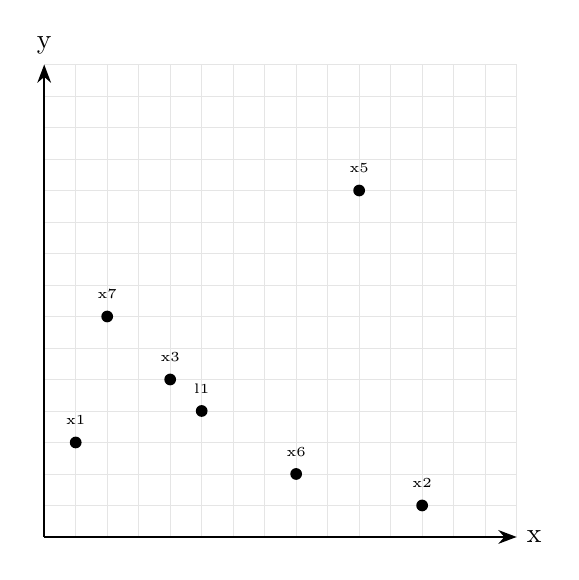
\begin{tikzpicture}[scale=0.4]
        % Grid
        \draw[very thin,gray!20] (0,0) grid (15,15);
        \draw[->,thick] (0,0) -- (15,0) node[right] {x};
        \draw[->,thick] (0,0) -- (0,15) node[above] {y};
        
        % Points with labels
        \node[circle,fill,inner sep=1.5pt] (x1) at (1,3) {};
        \node[font=\tiny] at (1,3.7) {x1};
        
        \node[circle,fill,inner sep=1.5pt] (x2) at (12,1) {};
        \node[font=\tiny] at (12,1.7) {x2};
        
        \node[circle,fill,inner sep=1.5pt] (x3) at (4,5) {};
        \node[font=\tiny] at (4,5.7) {x3};
        
        \node[circle,fill,inner sep=1.5pt] (x4) at (5,4) {};
        \node[font=\tiny] at (5,4.7) {l1};
        
        \node[circle,fill,inner sep=1.5pt] (x5) at (10,11) {};
        \node[font=\tiny] at (10,11.7) {x5};
        
        \node[circle,fill,inner sep=1.5pt] (x6) at (8,2) {};
        \node[font=\tiny] at (8,2.7) {x6};
        
        \node[circle,fill,inner sep=1.5pt] (x7) at (2,7) {};
        \node[font=\tiny] at (2,7.7) {x7};
    \end{tikzpicture}
    \caption*{Points in 2D plane}
\end{figure}

\begin{figure}[H]
    \centering
    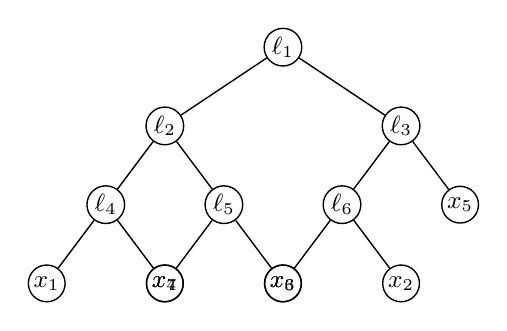
\begin{tikzpicture}[
        level distance=1cm,
        level 1/.style={sibling distance=3cm},
        level 2/.style={sibling distance=1.5cm},
        every node/.style={circle,draw,inner sep=1pt,font=\small}
    ]
        \node {$\ell_1$}
            child {node {$\ell_2$}
                child {node {$\ell_4$}
                    child {node {$x_1$}}
                    child {node {$x_4$}}
                }
                child {node {$\ell_5$}
                    child {node {$x_7$}}
                    child {node {$x_3$}}
                }
            }
            child {node {$\ell_3$}
                child {node {$\ell_6$}
                    child {node {$x_6$}}
                    child {node {$x_2$}}
                }
                child {node {$x_5$}}
            };
    \end{tikzpicture}
    \caption*{Final KD-Tree structure}
\end{figure}

\textbf{3. Answers:}
\begin{enumerate}[noitemsep]
    \item Height of the tree = 3 (counting levels from 0)
    \item Number of leaves = 7 (each original point becomes a leaf)
    \item Second leaf from left = $x_4 = (4,5)$
\end{enumerate}

\textbf{Key Insights:}
\begin{itemize}[noitemsep]
    \item The tree is built by alternating between x and y coordinates
    \item Each internal node represents a splitting line
    \item Vertical splits (even depths) compare x-coordinates
    \item Horizontal splits (odd depths) compare y-coordinates
    \item All original points end up as leaves
\end{itemize}

\subsection{Exercise 5.2: BUILDKDTREE Complexity}
\textbf{Problem:} (It is enough to give an intuitive idea) Prove that the BUILDKDTREE for a set of $n$ points has running time $O(n \log n)$ and uses $O(n)$ storage.

\textbf{Solution:} Let's break this down into two parts: storage complexity and runtime complexity.

\textbf{1. Storage Complexity $O(n)$:}
\begin{itemize}[noitemsep]
    \item Each splitting line divides points into two equal parts (up to unity)
    \item For $n = 2^k$ points, we need $2^k - 1$ lines (internal nodes)
    \item For splitting 2, the total nodes (parents + leaves) is:
        \[ 2^k + 2^{k-1} = n + n/2 = 3n/2 < 3n \]
    \item For $n$ not a power of 2, there exists $t$ where $2^{t-1} < n < 2^t$
    \item Number of internal nodes $n_p$ is bounded by:
        \[ 2^{t-2} < n_p < 2^{t-1} \]
    \item Total nodes (parents + leaves) satisfies:
        \[ 3 \cdot 2^{t-2} < n + n_p < 3 \cdot 2^{t-1} \]
    \item Therefore: $n + n_p < 3 \cdot 2^{t-1} < 3n$
    \item Each node uses $O(1)$ storage
    \item Total storage: $O(1) \cdot O(n) = O(n)$
\end{itemize}

\textbf{2. Runtime Complexity $O(n \log n)$:}
\begin{itemize}[noitemsep]
    \item BUILDKDTREE is recursive:
        \begin{itemize}[noitemsep]
            \item Each recursion splits $n$ points into two $n/2$ subsets
            \item Split cost is linear ($O(n)$): finding median in x or y coordinates
        \end{itemize}
    \item Building time $T(n)$ follows the recurrence:
        \[ T(n) = \begin{cases}
            O(1) & \text{if } n = 1 \\
            2T(n/2) + O(n) & \text{if } n > 1
        \end{cases} \]
    \item By Master Theorem (as in Merge-Sort):
        \begin{itemize}[noitemsep]
            \item $a = 2$ (subproblems)
            \item $b = 2$ (size reduction)
            \item $f(n) = O(n)$ (split cost)
            \item Case 1: $f(n) = O(n) = \Theta(n^{\log_2 2}) = \Theta(n)$
            \item Therefore: $T(n) = O(n \log n)$
        \end{itemize}
\end{itemize}

\textbf{Key Insights:}
\begin{itemize}[noitemsep]
    \item Storage is linear because each point becomes exactly one leaf node
    \item Runtime is $O(n \log n)$ due to:
        \begin{itemize}[noitemsep]
            \item Linear-time splitting at each level
            \item Logarithmic number of levels in the tree
        \end{itemize}
\end{itemize}

\begin{itemize}
    \item Example of a point $p_1$ \hfill
\end{itemize}

\begin{itemize}
    \item Example of a point $p_2$ \hfill
\end{itemize}

\begin{itemize}
    \item Example of a point $p_3$ \hfill
\end{itemize}

\begin{itemize}
    \item Example of a point $p_4$ \hfill
\end{itemize}

\begin{itemize}
    \item Example of a point $p_5$ \hfill
\end{itemize}


\end{document}